\documentclass{article}
\usepackage[utf8]{inputenc}
\usepackage{geometry}[margins = 1in]
\usepackage{graphicx}
\usepackage{hyperref}
\usepackage{eufrak}
\usepackage{fullpage}
\usepackage{amsmath}
\usepackage{listings}
\usepackage[makeroom]{cancel}
\usepackage{color}
\usepackage{amssymb}
\usepackage{float}
\floatplacement{figure}{H}
\setkeys{Gin}{width=0.75\linewidth}

\hypersetup{
    colorlinks=true, %set true if you want colored links
    linktoc=all,     %set to all if you want both sections and subsections linked
    linkcolor=blue,  %choose some color if you want links to stand out
}


\newcommand{\unit}[1]{{\,\rm #1}}
\newcommand{\be}{\begin{equation}}
\newcommand{\ee}{\end{equation}}
\newcommand{\Mpc}{\unit{Mpc}}
\newcommand{\s}{\unit{s}}
\newcommand{\km}{\unit{km}}
\newcommand{\yr}{\unit{yr}}


%%%%%
\def\:{\ddot }
\def\.{\dot }
\def\^{\hat }
\def\_{\bar }
\def\~{\tilde }
\def\hf{\frac12}
\def\imply{\Rightarrow}
\def\inv#1{\frac{1}{ #1}}
\def\ddt{\frac{d}{dt}}
\def\aa{\frac{\dot a }{ a}}
\def\adda{\frac{\ddot a}{ a}}
\def\thnot{\theta_0}
\def\etot{\Omega_0}
\def\econs{\Omega_{0,\Lambda}}
\def\emat{\Omega_{0,M}}
\def\econs{\Omega_{0,\Lambda}}
\def\p{^\prime}
\def\iff{\Leftrightarrow}
\def\xv{{\vec x}}
\def\pv{{\vec p}}
\def\vv{{\vec v}}
\def\ppt{\frac{\partial}{\partial t}}
\def\ddt{\frac{d}{dt}}
\def\epot{\frac{8\pi}{ 3}}
\def\attw{a^{3+3w}}
\def\athow{a^{-\frac{3}{2}(1+w)}}
\def\atow{a^{-3(1+w)}}
\def\atowi{a^{-3(1+w_i)}}



\title{Extragalactic Astrophysics and Comsology}
\author{Jacob Pilawa}
\date{Spring 2021}

\begin{document}

\maketitle
\tableofcontents
\newpage

\section{The Smooth Universe}
\subsection{The Cosmological Principle; The Hubble Parameter; Scale Factor}

\subsubsection{The Cosmological Principle}

We begin with \textbf{The cosmological Principle}. It sounds simple, but incredibly well supported. It says that \textbf{the Universe (spatially) is homogeneous and isotropic on very large spatial scales}. Observationally, this is around $100 \Mpc$ scales. Homogeneous means constant density (non-realistically, this is mass density; relativistic ally, this is energy density). Isotropic means the same in all directions. 

\textit{Note}: Isotropy about $2$ points (or more) implies homogeneity. Isotropy about $1$ point is not enough. Here is a quick illustration of that: 

\begin{figure}
    \centering
    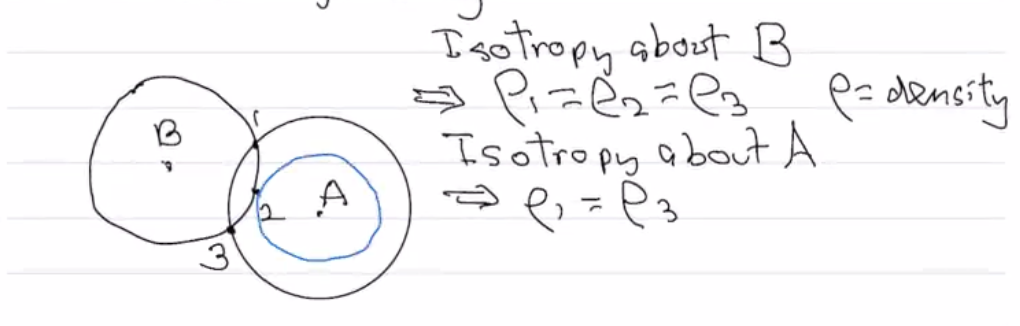
\includegraphics{isotropy.png}
    \caption{Istropy aobut 2 points.}
    \label{fig:isotropy}
\end{figure}

We can consider another example. A homogeneous universe can anisotropic. Consider a homogeneous Universe that is expanding in different directions in a non-uniform way. This leads to different $H_0(x,y,z)$. 

The reason we spend some time on the Cosmological Principle is the \textbf{Friedmann-Robertson-Walker metric}, which we will come to later on.

\subsubsection{Hubble Parameter}

Let's now talk about the \textbf{Hubble parameter}, which is not a constant! It, in fact, changes in time. An empirical linear relationship between the recession speed $v$ and distance $r$ can be seen, called the \textbf{Hubble's Law}:

\begin{equation}
v = H r
\end{equation}

Note that $H_0$ has units of $1/$time. One convention to note is that:

\begin{equation}
H = 100 \underbrace{h}_\text{to hide our ignorance} \frac{\km}{\s \Mpc}
\end{equation}

One useful number to know is $H \approx \frac{h}{10^{10} \yr}$.

Sometimes, when we write $H_0$, we mean the ``present-day'' value ($z = 0$). This is how we will use it now.

\subsubsection{Scale Factor}

We need a language to describe the expansion of the Universe. We will use $a(t)$, which describes the expansion (or contraction) of the Universe. It also relates two different coordinate systems: physical coordinates $\vec{r}$ to comoving coordinates $\vec{x}$. The relation:

\begin{equation}
    \vec{r} = a(t) \vec{x}
\end{equation}

We typically use comoving coordinates in calculations in Cosmology. We can think of $\vec{x}$ as the notches on a stretching ruler. Now consider:

\begin{equation}
    \frac{d}{dt}\vec{r} = \vec{v} = \dot{a} \vec{x} a \vec{\dot{x}}
\end{equation}

\begin{equation}
    \frac{d}{dt}\vec{r} = \vec{v} = \dot{a} \vec{x} a \vec{\dot{x}} = \underbrace{\frac{\dot{a}}{a} \vec{r}}_\text{Hubble} + \underbrace{a \vec{\dot{x}}}_\text{motion relative to expansion (``peculiar velocity'')}
\end{equation}

\begin{equation}
    \boxed{H(t) = \frac{\dot{a}(t)}{a(t)}}
\end{equation}

The name of the game for measuring $H$ is to go far enough that the first term dominates. Otherwise, locally, the second term dominates since peculiar velocities are of order $100$s of $\km/\s$. 

One other convention we need to establish:

\begin{equation}
    a(t_0) = 1 \rightarrow \text{comoving} = \text{today}
\end{equation}

\subsection{The Friedmann Equation; The Equation of State; Radiation, Matter, and Dark Energy}

\subsubsection{The Friedmann Equation}

Below, we will use and derive these, but I am putting the equations at the top for convenience. 

\begin{equation}
    \boxed{\left(\frac{\dot{a}}{a}\right)^2 = \frac{8\pi}{3} G \rho - \frac{k}{c^2}}
\end{equation}

\begin{equation}
    \boxed{\dot{\rho} = -3 \frac{\dot{a}}{a} \left(P + \rho\right)}
\end{equation}

\begin{equation}
    \boxed{\frac{\ddot{a}}{a} = - \frac{4\pi G}{3}\left(\rho +  3P\right)}
\end{equation}

Let's motivate the origin with quasi-Newtonian physics. We can derive it from General Relativity, but that's overkill.

If we assume isotropy, we only need to worry aobu the radial coordinate $r$, not $\theta$ or $\phi$. Homogeneity tells us that $\rho = \text{constant}$ spatially, but \textit{can} depend on time. We will model the Universe as an expanding, homogeneous medium that is adiabatically ($\Delta s =0$) expanding. If it were not adiabatically expanding, we would have heat flow and thus no isotropy. 

With these conditions, let's examine the motion of a thin, expanding, spherical shell of radius $a$. This depends \textbf{only} on the enclosed mass within $a$\footnote{see Birkhoff's Theorem for General Relativity proof}:


\begin{equation}
    M(<a) = \frac{4}{3}\pi a^3 \rho
\end{equation}

Let's consider the energy:


\begin{equation}
    E = \frac12 \dot{a}^2 - \frac{GM}{a}
\end{equation}


\begin{equation}
E = \frac12 \dot{a}^2 - \frac43 \pi G \rho a^2
\end{equation}

Let's re-write $E$ a bit: $k c^2 \equiv -2E$. Note that $k \propto 1/\text{length}^2$. There are three possibilities for $kc^2$:

\begin{itemize}
    \item $>0$, $E<0$, bound
    \item $=0$, $E=0$, critical
    \item $<0$, $E>0$, unbound
\end{itemize}

Let's now evoke the First Law of Thermodynamics ($\Delta S = 0$):

\begin{equation}
   \underbrace{\mathrm{d}U}_\text{internal energy} = -P \mathrm{d}V 
\end{equation}

We now equation the internal energy to the rest-mass energy:

\begin{equation}
    \mathrm{d}\left(\rho c^2 a^3\right) = -P \mathrm{d}\left(a^3\right)
\end{equation}

We will now set $c = 1$ and take a time derivative:

\begin{equation}
    \dot{\rho} a^3 + 3 \rho a^2 \dot{a} = -3P a^2 \dot{a}
\end{equation}

\begin{equation}
    \dot{\rho} -3\frac{\dot{a}}{a}\left(P + \rho\right)
\end{equation}

Using this result and the energy equation from above

\begin{equation}
    \left(\frac{\dot{a}}{a}\right)^2 = \frac{8\pi}{3}G \rho - \frac{k (c)^2}{a^2}
\end{equation}

to get a new equation. If you stare at it hard enough and have divine intervention, take a derivative of the second equation and multiply by $a^2$. Doing so, you get:

\begin{equation}
    2 \dot{a} \ddot{a} = \frac{8\pi}{3}G\frac{d}{dt}(\rho a^2) = \frac{8\pi}{3}Ga^2\left(\dot{\rho} + 2\frac{\dot{a}{a}}\rho\right)
\end{equation}

Simplifying with the other above equation, we get:

\begin{equation}
    2\dot{a}\ddot{a} = -\frac{8\pi}{3}Ga^2 \left(\frac{\dot{a}}{a}\rho + 3\frac{\dot{a}}{a}P\right)
\end{equation}

Simplifying:

\begin{equation}
    \frac{\ddot{a}}{\dot{a}} = -\frac{4\pi}{3}G \left(\rho + 3P\right)
\end{equation}

Note that this is not independent from the other equations; rather it is massaged. Let's compare this to $1$-D Newtonian forces:

\begin{equation}
    \ddot{x} = -\frac{GM}{x^2} = -\frac{4}{3}\pi G \rho x
\end{equation}

\begin{equation}
    \frac{\ddot{x}}{x} = -\frac{4}{3}\pi G \rho 
\end{equation}

Had we done strictly Newtonian physics, we would have never gotten the $+3P$ term. The way to interpret this: we can think of $\rho$ to have an extended meaning: $\rho_{eff} = \rho + 3P$. 

The Grand Summary so far: two equations of motion for $a(t)$: 

\begin{equation}
    \frac{\ddot{a}}{\dot{a}} = -\frac{4\pi}{3}G \left(\rho + 3P\right)
\end{equation}

\begin{equation}
    \dot{\rho}= -3\frac{\dot{a}}{a}\left(P + \rho\right)
\end{equation}

Note this second equation tells us the acceleration! Very importantly, we have a minus sign. If $\rho$ and $P$ are positive, the Universe is \textbf{decelerating}! Conversely, if you have a \textit{bizarre} $P$ and could reverse the parenthetical term, we can have accelerated expansion! 


Right now, we have three unknowns ($P, \rho, a$). How do we get that last piece -- the equation of state ($P \iff \rho$ dependence)?

\subsubsection{Equation of State}

We choose to write:

\begin{equation}
    P = w\rho (c^2)
\end{equation}

We are in units where $c = 1$, but I threw it in for reference. Note -- this means that pressure is the same thing as energy density! Think of the units. 

With that definition of $P$, we can re-write the second boxed equation from above:

\begin{equation}
    \dot{\rho} -3\frac{\dot{a}}{a}\left(1+w\right)\rho
\end{equation}

\begin{equation}
    \frac{\dot{\rho}}{\rho} = -3 (1+w) \frac{\dot{a}}{a} \rightarrow \rho \propto a ^{-3(1+w)}
\end{equation}

\begin{equation}
    \boxed{\rho \propto a^{-3\left(1+w\right)}}
\end{equation}

\textbf{assuming that} $\dot{w} =0$ \textbf{which might not be true}!

\subsubsection{Matter, Radiation, and Dark Energy}

Let's look at a few special cases of the equation of state:

\begin{itemize}
    \item Matter: Non-relativistic, pressure-less particles like cold dark matter. In this case, $w = 0, P = 0 \rightarrow \boxed{\rho \propto a^{-3}}$. This makes sense because it is units of $1/\text{volume}$.
    \item Radiation: Relativistic particles, photons and neutrinos. In this case, $w = 1/3, P = \frac13 \rho \rightarrow \boxed{\rho \propto a^{-4}}$. This makes sense because it is units of $\left(1/\text{volume}\right)\left(1/\text{length}\right) $ where the extra factor is from redshifting energy.
    \item The Cosmological Constant: In this case, $w = -1, P=-\rho \rightarrow \rho = \text{constant}$.
    \item Dark Energy: More general term, where $w < -\frac13$ to make $\ddot{a} >0$.
\end{itemize}

\begin{figure}
    \centering
    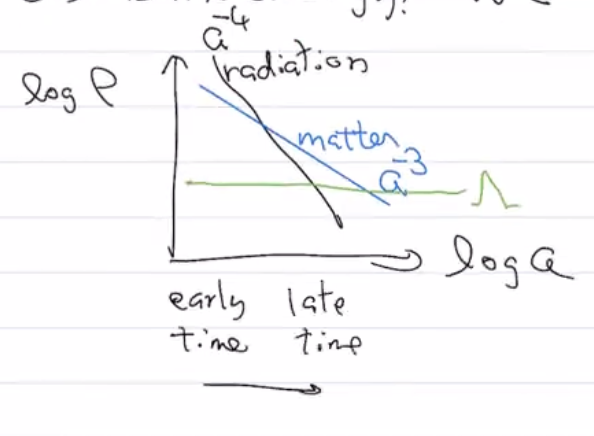
\includegraphics{density.png}
    \caption{Sketch of density over cosmic time. }
    \label{fig:density}
\end{figure}

\appendix 

\section{Archival Lectures (C.P. Ma)}

\subsection{Lecture 1}

\subsubsection*{ The Cosmological Principle}

The {\bf Cosmological Principle} states that the universe is spatially 
{\it isotropic} (looks the same in all directions) 
and {\it homogeneous} (has constant density everywhere) on large scales.
The {\bf Perfect Cosmological Principle} states that the universe is
also {\it temporally} isotropic and homogeneous (a steady state universe). 
This is unlikely because it doesn't describe the Cosmic Microwave Background
(CMB).  The CMB and Hubble's Law are both provide evidence for isotropy and
homogeneity.

\subsubsection*{ Hubble's Law (1929) }

Hubble's Law is an empirical law stating that, on large scales, recessional 
velocity is proportional to distance from observer.
$$\boxed{v=Hr}$$ 
where $H$, the Hubble parameter, is not constant, but can
vary slowly with time.  By convention, $H$ is often expressed as
$H=100\cdot h\frac{km}{ s\cdot Mpc}$, where 1 parsec (pc) $\approx3\cdot10^{18}cm
=3.26ly$, is the distance at which 1 AU appears as 1 arcsec on the sky.  
The Hubble Space Telescope Key Project (Freedman et al. ApJ 553, 47, 2001)
measured the present day value of Hubble Constant 
$H_0=72\pm 8\frac{km}{ s\cdot Mpc}$, giving us that the current timescale for
the expansion of the universe is 
$H_0^{-1}\approx\frac{h}{ 10^{11}}yrs\approx 9.778h^{-1}Gyrs$.

\subsubsection*{ The Scale Factor $a(t)$ }

$a(t)$ relates physical ($r$) and {\it comoving} ($x$) coordinates in an
expanding universe:
\begin{align}
r&=a(t)x\\
\dot r&=\dot ax+a\dot x=\underbrace{\aa}_{\equiv H}r+\underbrace{a\dot x}_{\equiv v_p}\\
\end{align}
Thus, the two components of physical velocity are $H$ (the Hubble expansion 
parameter) and $v_p$ (the peculiar velocity, or motion relative to expansion)
By convention, $t_0 \equiv$ today and $a(t_0)=1$.

\subsubsection*{ The Friedmann Equations}

The Friedmann Equation is an equation of motion for $a(t)$.  A rigorous
derivation requires General Relativity, but we can fake it with a
quasi-Newtonian derivation.
We will model the universe as an {\it adiabatically} ($\Delta S=0$) expanding,
isotropic, homogeneous medium.  Isotropy allows us to use $r$ as a scalar.
Consider a thin, expanding spherical shell of radius $a$.
Birkhoff's Theorum states that even in GR,
the motion of such a shell depends only on the enclosed mass 
$M={4\pi }{ 3}a^3\rho$.
Thus, the energy per unit mass per unit length is:
$$E=\overbrace{\hf \dot a^2}^{Kinetic}\overbrace{-\frac{G\cdot M}{ a}}^{Potential}
=\hf \dot a^2-\frac{4\pi }{ 3}G\rho a^2.$$
We define $k\equiv-\frac{2E}{ c^2}$, and we will show later that $k$ is a measure
of the curvature of the universe: 
$$k\begin{cases}
>0&\,for\ E<0\ (bound)\\
=0&\,for\ E=0\ (critical)\\
<0&\,for\ E>0\ (unbound)\\\end{cases}$$
where $k$ has units of $\inv{length^2}$ if $a$ is dimensionless.  Substituting
$k$ into the above energy equation, and solving for $\aa$, we get:
\def\paap{\left(\aa\right)}
$$\boxed{H^2=\paap^2=\epot G\rho -\frac{k c^2 }{ a^2}}$$
\centerline{($1^{st}$ Friedmann Equation)}
This is a statement of conservation of $E$.
The first law of thermodynamics ($\Delta S=0$) requires that any 
system with positive pressure must lose energy as the volume enclosing it
expands.  Thus, if $U$ is our internal energy and $P$ is our pressure:
$$\frac{dU}{ dt}=-P\frac{dV}{ dt}.$$  
In an expanding universe, $U={E}{ V}\cdot V=\rho a^3$, where $\rho$ is the
energy density of the universe.  $P$ is the pressure of the photon gas, so:
$$\dot \rho a^3+3\rho a^2\dot a=-P 3a^2\dot a,$$ 
which simplifies to:
$$\boxed{\dot \rho=-3\aa(\rho +P)}$$
\centerline{($2^{nd}$ Friedmann Equation)}
This is a a statement of the temperature loss of the universe 
due to adiabatic expansion.\par
Finally, $\ddt$($1^{st}$ Friedmann Equation) gives us:
$$2\dot a\ddot a=\epot G \frac{d }{ dt}(\rho a^2) =\epot G a^2(\dot \rho +2\aa \rho).$$
Substituting the $2^{nd}$ Friedmann Equation for $\dot \rho$:
$$2\dot a\ddot a=\epot Ga^2 (-\aa \rho -3 \aa P) =-\epot G \aa (\rho +3P).$$  
Now we have our $3^{rd}$ Equation:
$$\boxed{\frac{\ddot {a }}{ a}=-\frac{4\pi G} {3} (\rho + 3P)}$$
\centerline{($3^{rd}$ Friedmann Equation)}
The $3^{rd}$ Friedmann Equation relates the acceleration of the expansion of
the universe to the pressure of photon gas and the density of the universe.
Note that if $3P \le -\rho$, we have an accelerating universe.\par
Compare the $3^{rd}$ Friedmann Equation to the Newtonian equation for gravity,
with $M=\frac{4\pi }{ 3}\rho x^3$ and $\rho_{eff}=\rho +3P$:
$$\ddot x=\frac{-G\cdot M}{ x^2}={-4\pi }{ 3}G\rho x$$

\subsection{Lecture 2}

\subsubsection*{ The Friedmann Equations, continued }

Recall we had the following equations:
$$\paap^2={8\pi}{3}G\rho-\frac{k}{ a^2}$$
$$\dot \rho=-3\aa(\rho+P)$$
$$\frac{\ddot a}{ a}=-\frac{4\pi}{3}G(\rho+3P)$$

To close the equations, we need to relate $P$ and $\rho$ with an equation of
state:
$$\boxed{P=w\rho(c^2)}$$ 
Note that we will generally set $c=1$ in this class.
Combined with (2), this gives us:
\begin{align}
\dot \rho&=-3\aa(1+w)\rho\\
{\dot \rho}{\rho}&=-3(1+w)\aa\\
\rho&\propto\atow\\
\end{align}
Note that we've assumed $\dot w=0$, which is okay most of the time.
Some special cases of interest are:
\begin{itemize}
\item Pressure-less ``dust'' $P=0$, $w=0\imply\rho\propto a^{-3}$ because volume
goes as $V\propto\inv{a^3}$.
\item Relativistic particles (photons, bosons): $w=\inv{3}$, $P=\frac{\rho}{3}
\imply\rho\propto a^{-4}$ because $VV\propto\inv{a^3}$, and energy is given
by $E\propto\inv{a}$.
\item  ($\Lambda$)/Dark Energy: $w=-1$, $P=-\rho\imply\rho=$ constant 
in time.
\end{itemize}
To get density ($\rho$) as a function of time, want to solve for $w$.

\subsubsection*{ Critical Density, $\rho_{crit}$ }

We define $\rho_{crit}$ to be the critical density at which $k=0$ (and $E=0$):
\def\rcr{{\rho_{crit}}}
$$\rcr=\frac{3H^2}{8\pi G}$$
Today, we measure: $\rho_{crit,0}=\frac{3H_0^2}{8\pi G}= 
\frac{3}{8\pi}\frac{\left(100h\frac{km}{ sMpc}\right)^2}{ G}=2.78\cdot10^{11}h^2
\frac{M_\odot}{ Mpc^3}=1.88\cdot10^{-29}h^2\frac{g}{ cm^3}$.
Note that the mass of the sun is $M_\odot=2\cdot10^{33}g$, and
the mass of the proton is $M_p=1.67\cdot10^{-24}g$.

\subsubsection*{ Density Parameter, $\Omega(t)$}

$\Omega$ measures the ratio of the density of the universe to the critical
density:
$$\Omega(t)\equiv\frac{\rho(t)}{\rho_c(t)}=\frac{8\pi G\rho(t)}{ 3H^2(t)}$$
$$\Omega\begin{cases}
\le1&\imply open\ (k\le0)\\
=1&\imply flat\ (k=0)\\
\ge1&\imply closed\ (k\ge0)
\end{cases}$$

In general, $\Omega$ can consist of multiple components: 
$\Omega=\sum_i{\Omega_i}$ e.g. 
$$\Omega\begin{cases}
r&=radiation\\ 
m&=matter\ (dark\ and\ luminous)\\
b&=baryons\ (dark\ and\ luminous)\\ 
\nu &=neutrinos\\ 
\Lambda&=dark\ energy\end{cases}$$

$\Omega = 1$ is an unstable equilibrium; any perturbation from $\Omega=1$ in
the early universe ensures $\Omega$ is far from 1 today.  That we measure
$\Omega_m\approx0.3$ today implies that the early universe must have been
extremely finely tuned.

\subsubsection*{ Evolution of $H(t)$}

Today (at $a=1$): $k=\epot G\rho_0-H_0^2=H_0^2(\Omega_0-1)$.  Using the
$1^{st}$ Friedmann equation (1), we have:
$$\boxed{H^2=H_0^2(\frac{\Omega_0}{ a^{3+3w}}+\frac{1-\Omega_0}{ a^2})}$$
\centerline{\bf (THE Friedmann Equation)}
where $H_0\equiv\sqrt\frac{8\pi G\rho}{3\rcr}$, and it is understood that
$\etot=\sum_i{\Omega_{i,0}}$.  Each $\Omega_i$ has it's own $w_i$, so really
$\frac{\Omega_0}{\attw}=\sum_i\frac{\Omega_{i,0}}{ a^{3+3w_i}}$.

\subsubsection*{ Evolution of $\Omega(a)$}

We'll show in PS\#1 that for any single component:
$$\frac{1-\Omega(a)}{\Omega(a)}=\frac{1-\Omega_0}{\Omega_0}a^{1+3w}$$
Plotting $\Omega(a)$, we will find that for early $a$, $\Omega$ is {\it 
extremely} close to 1.

\subsubsection*{ Evolution of $a(t)$: Solving the Friedmann Equation}

The evolution of the expansion of the universe is governed by:
$$\paap^2=\epot G\rho-\frac{k}{ a^2}$$

We can apply this to several models of the universe:
\begin{itemize}
\item The Einstein-deSitter (flat) Model: $k=0$, $\Omega(a)=\Omega_0=1$.
Using that $\rho\propto\atow$, we have:
\begin{align}
\paap^2&\propto\atow\\
a^{-1}a^{{3}{ 2}(1+w)}da&\propto dt\\
\athow&\propto t\\
\end{align}$$
$$\boxed{a(t)\propto t^{{2}{ 3(1+w)}}}
Thus, the rate of expansion of the universe depends on $w$:
\item{(a)} The matter-dominated era: 
$\Omega\approx\Omega_m\imply w=0, P=0, a\propto t^\frac{2 }{ 3}$.
\item{(b)} The radiation-dominated era: 
$\Omega\approx\Omega_r\imply w=\inv{3} \imply a(t)\propto t^\hf$.
\item{(c)} The $\Lambda$-dominated era: 
$\Omega\approx\Omega_\Lambda\imply w=-1, P=-\rho, \rho$ constant in time
$\imply a(t)\propto e^{Ht}$, where H is now actually a constant.  This
is exponential inflation.  We used to think that this only happened early on 
(like $10^{-34}$
seconds), but now we think that this has also been happening recently.
Next time, we will do the harder two cases: open and closed.
\end{itemize}

\subsection{Lecture 3}

\subsection{Lecture 4}

\subsection{Lecture 5}

\subsection{Lecture 6}

\subsection{Lecture 7}

\subsection{Lecture 8}

\subsection{Lecture 9}

\subsection{Lecture 10}

\subsection{Lecture 11}




\end{document}
